\begin{frame}{Travelling Salesman Problem Definition}
\begin{minipage}{0.45\textwidth}
  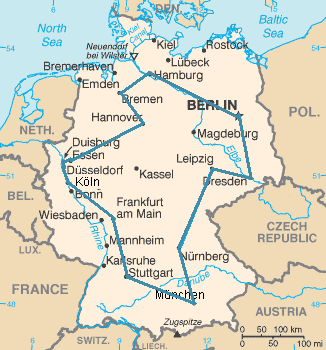
\includegraphics[width=0.8\textwidth]{TSP_Deutschland_3}
  \tiny

  user "Kapitän Nemo" \url{https://commons.wikimedia.org/w/index.php?curid=5584283}
\end{minipage}
\begin{minipage}{0.45\textwidth}

"Given a list of cities and the distances between each pair of cities, what is the shortest possible route that visits each city exactly once and returns to the origin city?"
\cite{song_solving_2021}
\end{minipage}
\end{frame}

\begin{frame}{Travelling Salesman Problem Definition}
  \begin{itemize}
    \item input graph
      \begin{itemize}
        \item weighted, non-negative
        \item undirected
        \item complete (fully connected)
      \end{itemize}

    \pause
    \item output restrictions:
      \begin{itemize}
        \item tour (cycle that visits every vertex)
        \item use any edge \emph{at most} one time
      \end{itemize}
    \pause
    \item problem: find a legal output that has minimal (cumulative) edge weight
  \end{itemize}
  \pause
  note: we do not assume the triangle inequality
\end{frame}

\begin{frame}{Why is TSP interesting?}
  \begin{itemize}
    \item well studied
    \item NP-complete $\rightarrow$ ressource intensive
    \item intuitive to understand
    \pause
    \item practical applications (see \href{https://en.wikipedia.org/wiki/Concorde_TSP_Solver}{Concorde TSP Solver})
  \end{itemize}
  % https://upload.wikimedia.org/wikipedia/commons/c/c4/TSP_Deutschland_3.png
\end{frame}
